\documentclass{article}

\title{Sprawozdanie z baz danych}
\author{Artur Dziedziczak}
\date{\today}

\usepackage[
    backend=biber,
    natbib=true,
    url=true, 
    doi=true,
    eprint=false
]{biblatex}

\addbibresource{sample.bib}
\usepackage{gensymb}
\usepackage{graphicx}
\usepackage{minted}
\usepackage[a4paper, total={6in, 8in}]{geometry}

\usepackage{hyperref}
\hypersetup{
    colorlinks=true,
    linkcolor=blue,
    filecolor=magenta,      
    urlcolor=cyan,
    pdftitle={Overleaf Example},
    pdfpagemode=FullScreen,
    }
    
\usepackage{float}

\usepackage[utf8]{inputenc}
\usepackage{amsthm}
\usepackage[english, polish]{babel}
\usepackage[T1]{fontenc}
\usepackage{theorem}

\begin{document}

\maketitle

\section{Temat pracy}

System do zarządzania flotą samochodów ciężarowych

\section{Zadanie 1}
 Historyjki użytkownika:

\begin{enumerate}
    \item Jako kierowca chcę mieć możliwość sprawdzenia gdzie ostatnio zaparkowałem pojazd żeby móc go odnależć.
    \item Jako szef chcę wiedzieć ile samochodów jest obecnie gotowych do pracy tak abym mógł lepiej zaplanować koszty amortyzacji.
    \item Jako pracownik biura chciałbym mieć możliwość monitorowania czy pracownik oddał samochód na czas tak abym mógł określić jego przyszłą wypłatę przez liczbę przepracowanych godzin.
    \item Jako kierowca chcę wiedzieć kto przede mną używał pojazdu tak abym mógł zgłosić nieprawidłowości stanu.
    \item Jako zewnętrzna firma obsługująca monitorowanie pojazdów firmy chielibyśmy mieć możliwość zapisywania ostatniej pozycji pojazdu co 15 min tak aby w przyszłości łatwiej móc określić pozycję pojazdu po jego uruchomieniu.
\end{enumerate}

\section{Zadanie 2}
Baza danych w schemacie ERD bez tabel łączących jest prosta ale pozwoli na 
realizację rozbudowanych akcji, które są zawarte w historyjkach użytkownika.

\begin{figure}[H]
    \centering
    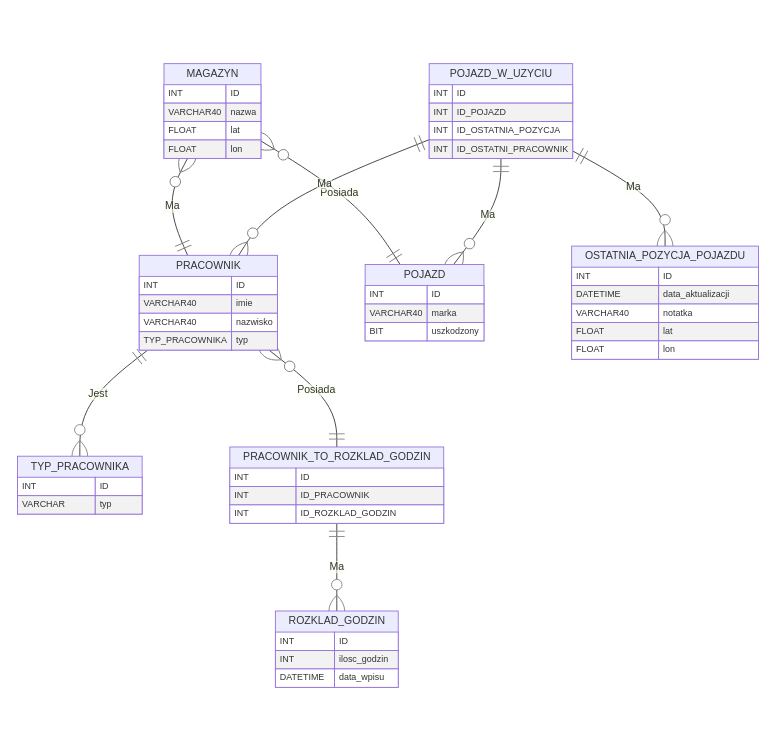
\includegraphics[width=\textwidth]{assets/chart.png}
    \caption{Schemat ERD bazy danych przed implementacją.}
\end{figure}

Zasadniczo baza składa się z 4 tabel głównych i jednej uzupełniającej \textbf{TYP\_PRACOWNIKA}. 

\begin{itemize}
    \item \textbf{MAGAZYN} - przechowuje informacje o magazynie, który może posiadać
        pracowników oraz samochody. 
    \item \textbf{POJAZD} - przechowuje informacje o pojeździe. Każdy pojazd posiada
        markę i status czy jest zdolny do jazdy.
    \item \textbf{OSTATNIA\_POZYCJA\_POJAZDU} - przechowuje informację o ostatniej pozycji pojazdu. W samej implementacji relacja pomiędzy \textbf{POJAZD} - \textbf{OSTATNIA\_POZYCJA\_POJAZDU} zostanie rozwinięta o tabelę \textbf{POJAZD\_W\_UZYCIU}, która będzie również zawierała informację o kierowcy danego samochodu.
    \item \textbf{PRACOWNIK} - przechowuje informacje o pracowniku.
    \item \textbf{ROZKLAD\_GODZIN} - przechowuje informacje o czasie pracy pracowników.
        Taki czas pracy składa się z ilości godzin przepracowanych danego dnia.
        Każdy \textbf{PRACOWNIK} danego dnia może dodać więcej niż jeden wpis gdyż
        pracownicy mogą pracować w różnych godzinach.
    \item \textbf{TYP\_PRACOWNIKA} - przechowuje informacje o typie pracownika. Typy wymagane to \textbf{szef, kierowca, biuro}.
\end{itemize}

\section{Zadanie 3 - Tabele}

\begin{figure}[H]
    \centering
    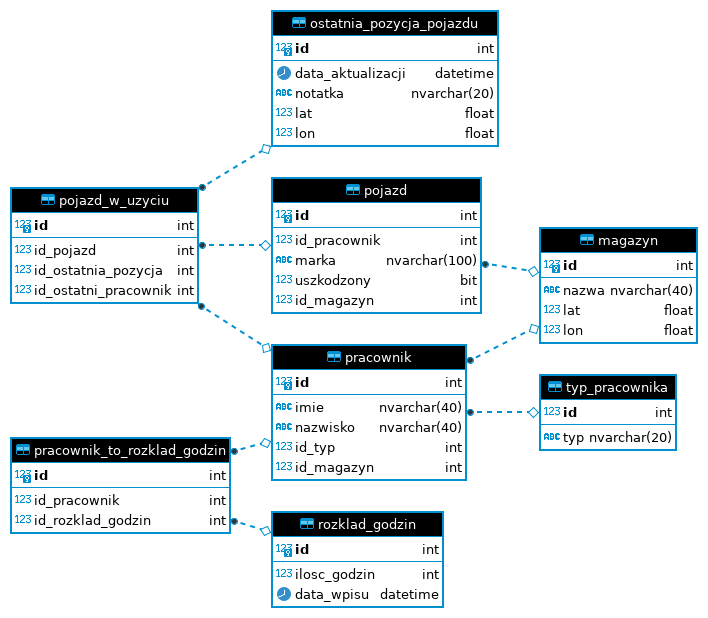
\includegraphics[width=\textwidth]{assets/chart-after-implementation.png}
    \caption{Schemat ERD bazy danych po implementacji.}
\end{figure}

Diagram różni się odrobinę od tego przed implementacją. Główną różnicą jest
wprowadzenie tabeli, które pozwalają na relację wiele do wielu i jeden do wielu.
Z tego samego powodu również atrybuty uległy zmianie.

Poniżej zamieszczam kod budujący bazę danych. 

\textbf{\textcolor{orange}{Do sprawdzenia bezy w SQL server bardzo proszę 
o używanie plików zad3.sql, zad4.sql, zad5.sql gdyż LaTeX z paczką minted
dodaje specjalne znaki do kodu gdy jest on załamywany.}}

\inputminted[breaklines, breaksymbolleft=]{sql}{../zad3.sql}

\section{Zadanie 4 - Procedury}

Poniższy kod ilustruje procedury, które realizują niektóre przypadki użycia.
Przypadki te są umieszczone w komentarzach.

\inputminted[breaklines, breaksymbolleft=]{sql}{../zad4.sql}

\section{Zadanie 5 - Widoki}
\inputminted[breaklines, breaksymbolleft=]{sql}{../zad5.sql}

\section{Jak uruchomić}

Najpierw należy uruchomić \textbf{zad3.sql}, które buduje bazę danych.
Następnie \textbf{zad4.sql} z procedurami a na koniec \textbf{zad5.sql}
plik z widokami.

\end{document}
